\section{Experiment}

In this section we explore the results of a Python implementation of $\beta$-VAE on a toy EMNIST (extension to MNIST) dataset of handwritten digits and characters. The code can be found here: \url{https://github.com/benlevyx/beta-vae}.

\subsection{Model architecture and dataset}

We use the EMNIST dataset, which is an image dataset similar to MNIST, except that it also includes handwritten letters \cite{cohen2017emnist}. Each digit is $28\times 28$ pixels with a single grayscale channel. The dataset includes handwritten digits from 0 to 9 and letters from a to z, including lowercase and uppercase. For simplicity, we take a subset of the data comprising the letters A through D (uppercase and lowercase).

The model encoder and decoder both consist of feed-forward neural networks. The 2D images are flattened to a vector of 784, which are then fed into the network in batches of 256 for computational efficiency. Since the goal of this experiment is to be able to plot the low-dimensional representations of the data for different levels of $\beta$, we use a latent dimension $d=2$. We train models with $\beta=0.0, 1.0, 5.0$ for 15 epochs each using the Adam optimizer with learning rate $10^{-3}$.

\begin{figure}[h!]
    \centering
    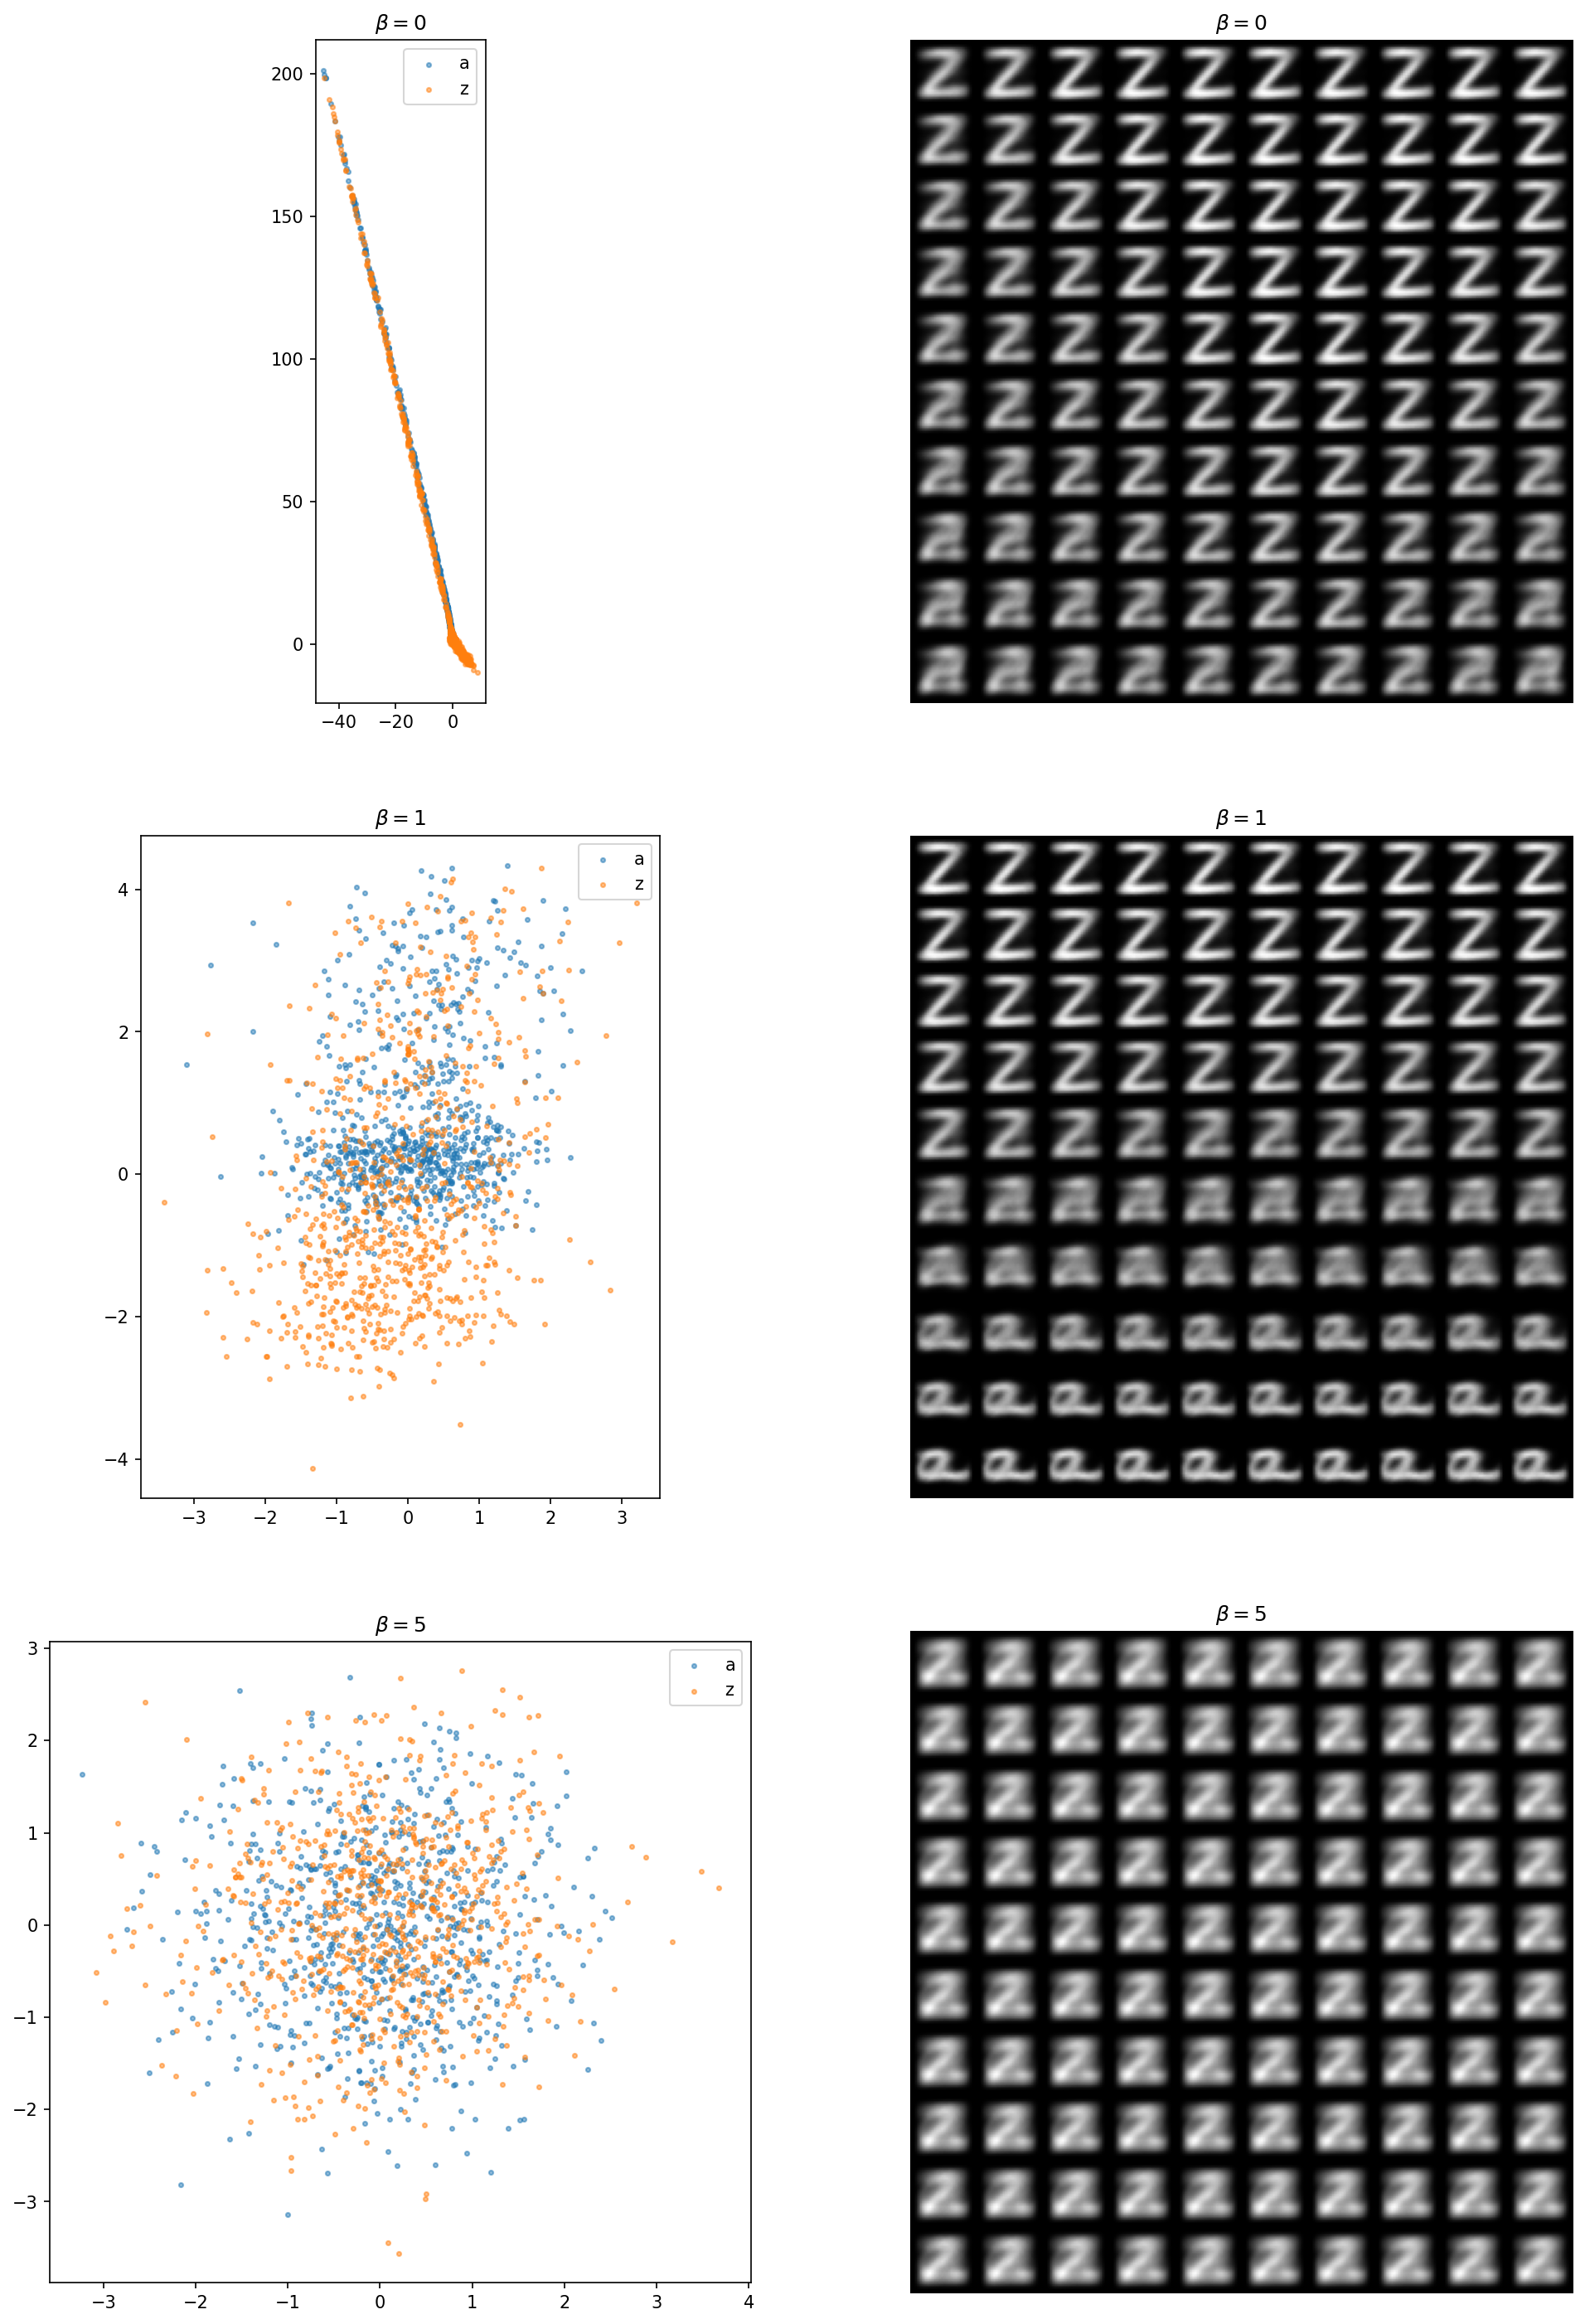
\includegraphics[width=0.7\textwidth]{beta-vae-experiment}
    \caption{Results from experiment with different levels of $\beta$. Each row represents a model trained with a different level of $\beta$. The left column plots the 2-dimensional representation of the evaluation data, colour-coded according to whether the point is an `A' or `Z'. The right column shows a traversal of the latent space in the fixed range $(-4,4)$ for both latent dimensions.}
    \label{fig:beta-vae-experiment}
\end{figure}

\subsection{Effect of $\beta$ on latent space}

In figure \ref{fig:beta-vae-experiment}, we can see the effect of $\beta$ on the latent space. The starkest difference is between $\beta=0$ and the cases where $\beta > 0$. In the former, we see that the latent space is extended along a line such that each point is essentially assigned its own location in that latent space. This resembles the latent space for a non-Bayesian autoencoder, since the model is only incentivized to reconstruct the data faithfully and is not encouraged to learn a smooth latent space.

As $\beta$ increases, we see that the latent space becomes closer to a standard Gaussian distribution. This is a double-edged sword: althouh the latent space is smoother and perhaps generalizes better, we completely lose the ability to discriminate between the two classes.

Of course, this is an extreme case meant to illustrate the effect of strong and weak regularization on the geometry of the latent space. In the real world, we would implement a $\beta$-VAE with a larger bottleneck dimension (2 is quite extreme), which would also allow for more fine-tuning of $\beta$.